\chapter{Support-Vector-Machines}
\usetikzlibrary{calc}
\usetikzlibrary{positioning}
\usetikzlibrary{matrix}

\section{Intro \& Motivation}
Obwohl keine allgemein anerkannte Definition von Intelligenz in Menschen (oder
Tieren) existiert, ist durchaus Konsens über wichtige Merkmale intelligenten
Verhaltens gegeben. So gut wie allen Definitionsversuchen ist gemein, dass Intelligenz
mit der Fähigkeit einhergeht, sich in einer sich ändernden Umwelt zurechtzufinden
und der Fähigkeit schnell zu lernen. Im Allgemeinen findet Lernen und die Adaptation
an Umweltgegebenheiten zum Erreichen bestimmter Ziele statt. Legg und Hutter
$($2007$)$ schlussfolgern in ihrer Sammlung verschiedener Definitionsversuche:

\begin{quote}
``Intelligence measures an agent’s ability to achieve goals in a wide range of
  environments. Features such as the ability to learn and adapt, or to understand,
  are implicit in the above definition as these capacities enable an agent to succeed
  in a wide range of environments.''
\end{quote}

Da bestimmte physikalische Prozesse immer chaotisch, das heißt nicht deterministisch,
ablaufen, können nicht alle Veränderungen von Umweltbedingungen vorausgesagt
werden. Ein intelligentes System muss demnach notwendigerweise mit Unsicherheit umgehen
können, um sinnvoll zu handeln $($Lawrence, 2016$)$. Es ist nicht möglich einem
intelligenten System die Voraussetzungen für alle möglichen zukünftigen Entwicklungen
mit auf den Weg zu geben. Wenn es nicht lernen kann, ist es kein intelligentes
System.  Die Fähigkeit sich auf neuartige Umgebungen einzustellen ist also essentiell
für intelligentes Verhalten. Die Voraussetzung für eine solche Anpassung ist eine
sehr allgemeine Fähigkeit aus Erfahrung und Beobachtung zu lernen -- Lernen ist der
Mechanismus, der eine individuelle Adaptation ermöglicht. Eine weitere Voraussetzung
für intelligentes Lernen ist das Vorhandensein eines oder mehrerer Ziele, die
bestimme,n aus welchen Informationen überhaupt gelernt werden soll.

Ein intelligentes, anpassungsfähiges System muss also einen Lernmechanismus besitzen,
mit dem das System sich selber verbessern, zeitüberdauernd Ziele verfolgen und den
Erreichungsfortschritt überwachen kann. Dies ist gerade dann relevant, wenn sich
gegebene Umweltbedingungen verändern und Handeln angepasst werden muss. Wenn
beispielsweise ein Computersystem überwachen soll, was für Situationen mit hoher
Wahrscheinlichkeit zu einer Gefährdung des Straßenverkehrs führen, muss das System
etwaige Änderungen in den Rahmenbedingungen -- zum Beispiel technologische
Erneuerungen, Änderungen der gesetzlichen Bestimmungen oder Änderungen des
Verkehrsaufkommens -- in seiner zukünftigen Vorhersage berücksichtigen. Das System
muss durch Lernen aus Beobachtung einschätzen, welchen Gegebenheiten mit dem
Auftreten von Unfällen zusammenhängen, um für die Zukunft Vorhersagen zu erstellen
und gegebenenfalls Interventionsmaßnahmen einzuleiten.

\section{Arten des maschinellen Lernens}
Es gibt verschiedenen Klassifikatoren, die dazu genutzt werden um Proben in einem mehrdimensionalen Raum Klassen zuzuordnen.
Dabei kann man Klassifikatoren in drei Arten unterscheiden.
\begin{enumerate}
\item Unüberwachtes Verfahren: Klassen müssen vom Klassifikator erkannt werden.
\item Überwachtes Vefahren: Klassen werden vorher in einer Trainingsphase erlernt.
\item Bestärkendes Verfahren: Klasseneinteilung ist nicht fest und wird durch hinzufügen von Informationen korrigiert.
\end{enumerate}
Dabei gehört die Support Vector Machine zu Art zwei. Zuerst wird eine Trainingsphase durchlaufen anhand der Klassifikator lernt, die Klassen zu unterscheiden. Nach der Trainingsphase können neue Daten mit Hilfe eines erstellten Modells zu einer der beiden Klassen zugewiesen werden.

Die folgende Ausarbeitung beschäftigt sich mit den Grundlagen statistischen Lernens,
welches maschinellen Systemen das Lernen aus Beobachtung ermöglicht. Hierbei gehe ich
vor allem auf das sogenannte \emph{überwachte Lernen} ein und beziehe mich in erster
Linie auf die Quellen \emph{Artificial Intelligence -- A Modern Approach} $($3. Ed.,
Kap. 18; Russel \& Norvig, 2010$)$ und \emph{An introduction to Statistical
  Learning} $($James, Witten, Hastie \& Tibshirani, 2013$)$.

\section{Lernen aus Daten}

Damit ein System intelligent lernen kann, müssen Beobachtungen in ein Format gebracht
werden, mit dem das System umgehen kann. Menschen und Tiere besitzen primäre
Sinnesorgane, die Informationen über die Umwelt über Nervenlaufbahnen in ein
zentrales Nervensystem transferieren. Dort werden Informationen aus verschiedenen
Sinnesmodalitäten integriert und Handlungen geplant; vereinfacht gesagt liegen
Informationen in Form von Nervenimpulsen vor. Ein Computersystem muss Informationen
über die Umwelt in einem quantifizierten, numerischen Datenformat erhalten. Auch
Daten, die distinkte, qualitative Merkmale repräsentieren -- beispielsweise die
Marke eines Autos -- werden dem Computersystem in numerischer Form übergeben.

Beim sogenannten überwachten Lernen (\emph{supervised learning}) werden Daten
allgemein im folgenden Format dargestellt: Betrachtet werden \emph{n} Datenpaare


\begin{equation*}
    (x_{1}, y_{1}), (x_{2},y_{2}), \ldots, (x_{n}, y_{n}).
\end{equation*}

Hierbei bezeichnen $x_{i}$, die \emph{Input}-Variablen, $y_{i}$
die \emph{Output}-Variablen. $X_{i}$ ist dabei entweder ein einzelner Wert
oder ein Vektor beliebig vieler Werte. Eine Input-Variable könnte beispielsweise die
Geschwindigkeit eines Autos, die Automarke oder das Temperament und Geschlecht des
Autofahrers darstellen. Ziel des überwachten Lernens ist mithilfe der vorhandenen
Input-Variablen (auch genannt: Features, Prädiktoren, unabhängige Variablen)
zuverlässige Informationen über den Output (auch genannt: abhängige Variablen,
Labels) zu erlangen.

Die Output-Werte y könnten beispielsweise repräsentieren, ob ein
Auto am Tag der Datenaufzeichnung einen Unfall hatte. Dies stellt ein qualitatives
Label dar: die Variable nimmt zwei distinkte Zustände an, entweder \emph{Unfall --
  Ja} oder \emph{Unfall -- Nein} (im Computer dargestellt als 1 / 0). Probleme, in
denen solch ein qualitativer Output vorhergesagt werden soll, werden
\textbf{Klassifikationsprobleme} genannt; existieren genau zwei qualitative
Kategorien, handelt es sich um ein \emph{binäres} Klassifikationsproblem. Angenommen,
das System soll nicht vorhersagen, ob Autos genau am Tag der Aufzeichnung einen
Unfall haben. Schließlich ist für ein einzelnes Auto das Auftreten eines Unfalls sehr
selten und die Variable ist somit wahrscheinlich nicht sehr informativ. Trotzdem soll
das System eine Prognose für die Fahrsicherheit eines jeden beobachteten Autos
ausstellen, damit in Zukunft riskante Verkehrssituationen mit hoher Präzision
eingeschätzt werden können. In diesem Fall könnte als Output die Fahrstrecke, die ein
Auto nach der Aufzeichnung noch unfallfrei fährt, dienen. Die Fahrstrecke stellt eine
kontinuierliche Variable dar -- es werden nicht qualitativ verschiedene Kategorien
betrachtet. Mit der Vorhersage kontinuierlicher Variablenwerte beschäftigen sich die
sogenannten \textbf{Regressionsprobleme}. Tabelle 2.1 zeigt einige exemplarische
Input- und Outputwerte für das Regressionsproblem unseres Fahrsicherheitssystems.

\begin{table}[h!]
  \centering
  \caption{Beispielhafte Input- und Outputwerte für das Fahrsicherheitssystem.}

\vspace{0.3cm}

  \label{tab:svm_table1}
  \def\arraystretch{1.5}%
  \begin{tabular}{l|c|c|c||c|c}
    & Automarke & Geschwindigkeit & Laune & Unfallfreie Fahrstrecke &\\
    \hline
    x\textsubscript{1} & Volvo & 73 km/h & fröhlich & 14,302 km & y\textsubscript{1}\\
    \hline
    x\textsubscript{2} & VW & 144 km/h & neutral & 10,219 km & y\textsubscript{2}\\
    \hline
    x\textsubscript{3} & Audi & 129 km/h & traurig & 21,219 km & y\textsubscript{3}\\
    \hline

    & ... & ... & ... & ... &\\
    \hline
    x\textsubscript{n} & Porsche & 267 km/h & wütend & 22 km & y\textsubscript{n} \\

  \end{tabular}
\end{table}

\vspace{0.3cm}

Beim unüberwachten Lernen (\emph{unsupervised learning}) liegen keine Informationen
bezüglich möglicher Output-Variablen vor -- hier wird alleine in den Input-Variablen
nach Gesetzmäßigkeiten gesucht, um die Daten auf bestimmte Art und Weise zu
strukturieren oder klassifizieren. Dies wäre in unserem Beispiel der Fall, wenn gar
keine Information bezüglich des Auftretens von Unfällen vorliegen würden. Die
vorhandenen Daten könnten trotzdem nach systematischen Regelmäßigkeiten untersucht
werden, etwa mittels \emph{Clustering}. Beispielsweise könnte sich herausstellen,
dass männliche Fahrer in Sportwagen generell jähzorniger sind als weibliche
Fahrerinnen in Kleinwagen -- ohne, dass man dies zuvor explizit erwartet hätte.

Im semi-überwachten Lernen existieren zu manchen Datenpunkten (x\textsubscript{i},
y\textsubscript{i}) Outputwerte y, aber für manche nicht. Dies wäre beispielsweise
der Fall, wenn die Datensammlung nicht lange genug gegangen ist, um für alle
beobachteten Autos die Fahrdistanz bis zum nächsten Unfall zu beobachten.

\subsection{Überwachtes Lernen}

Beim überwachten Lernen wird generell angenommen, dass y durch die Prädiktoren X =
(x\textsubscript{1}, x\textsubscript{2}, ..., x\textsubscript{n}) beschrieben werden
kann. Dabei soll es eine wahre Funktion $f$ geben, die y in Abhängigkeit von X
darstellt:

\begin{equation*}
y = f(X)
\end{equation*}


Ziel des überwachten Lernens ist es eine Funktion \emph{h} zu finden, welche die
wahre Funktion \emph{f} möglichst gut approximiert -- das intelligente System soll
\emph{f} lernen, indem verschiedene Kandidaten-Funktionen untersucht werden. Diese
Form des Lernens wird auch \emph{induktives Lernen} genannt: aus beobachteten
Phänomenen sollen allgemeine Regeln abgeleitet werden, durch die die Beobachtungen
erklärt werden können. Da die wahre Funktion \emph{f} im Allgemeinen unbekannt ist
und nicht bestimmt werden kann, ist man in der Praxis häufig daran interessiert eine
solche Funktion \emph{h} zu bestimmen, die y möglichst fehlerfrei vorhersagt. Zu
diesem Zweck werden die untersuchten Funktionen an einem Trainingsdatensatz
trainiert und die Vorhersagegüte wird dann an einem unabhängigen Testdatensatz
überprüft. Ziel ist es, den Testdatensatz anhand der Passung, die am
Trainingsdatensatz erstellt wurde, möglichst gut vorherzusagen.  Ob die Funktion
\emph{h} der wahren Funktion \emph{f} ähnelt, ist zumeist gar nicht so wichtig
solange sie akkurate Vorhersagen bezüglich der Zustände der Outputvariablen macht. In
Klassifikationsproblemen kann die Vorhersagegüte einfach durch den prozentualen
Anteil aller falschen Zuordnungen angegeben werden. Im Fall binärer Entscheidungen
kann die Korrektheit von Entscheidungen mit einer 2x2 Tabelle dargestellt werden:

\begin{table}[h!]
  \centering
  \caption{Entscheidungsmöglichkeiten in einer binären Klassifikationsaufgabe.}

\vspace{0.3cm}
  \def\arraystretch{1.5}%
  \label{tab:svm_table2}
  \begin{tabular}{c|c|c}
     & Status: Unfall & Status: kein Unfall \\

 \hline
    \parbox[t]{2.2cm}{Vorhersage:\\ Unfall\\}
    & \parbox[t]{2.2cm}{richtige\\Klassifikation \\}
    & \parbox[t]{2.2cm}{falsche\\Klassifikation \\} \\

 \hline
    \parbox[t]{2.2cm}{Vorhersage:\\ kein Unfall\\}
    & \parbox[t]{2.2cm}{falsche\\Klassifikation \\}
    & \parbox[t]{2.2cm}{richtige\\Klassifikation \\} \\


  \end{tabular}
\end{table}

\vspace{0.3cm}

In Regressionsproblemen ist die einfache Vorhersage-Trefferrate kein sinnvolles
Gütekriterium für die Passung einer Funktion. Angenommen, \emph{h} bestimmt für einen
Fahrer eine unfallfreie Fahrt von 1,237.47 Kilometer, das Auto hat den nächsten
Unfall aber nach 1,237.48 km -- die Vorhersage liegt sehr nah am tatsächlichen Wert,
ist aber nicht korrekt. Ist diese Abweichung als problematisch zu betrachten?  Wäre
eine Vorhersage von 20,000 km "`gleich falsch"'? Es macht Sinn in diesem Fall den
Schweregrad der Abweichung der Vorhersage zu berücksichtigen. Bei kontinuierlichem
Output wird deswegen der Vorhersagefehler durch die Abweichungen der vorhergesagten
von den tatsächlichen y-Werten bestimmt. Dabei wird häufig die mittlere quadratische
Abweichung (\emph{mean squared error}; MSE) als Fehlermaß verwendet.

\vspace{0.3cm}

$MSE=\displaystyle \frac{1}{n} \displaystyle \sum_{i=1}^{n} (y_i - h(x_i))^2$

\vspace{0.3cm}

Hierbei sind y\textsubscript{i} die beobachteten Output-Werte und
\emph{h}(x\textsubscript{i}) die vorhergesagten Werte auf Basis der zugehörigen
Input-Werte.

Die Funktion \emph{h} sollte so gewählt werden, dass die Vorhersagefehler
gering gehalten werden. Tatsächlich wird aber bei der Wahl von \emph{h} nicht nur die
Fehlerrate minimiert, sondern die \textbf{Kosten} verschiedener Fehlentscheidungen
können ebenfalls berücksichtigt werden. Nicht alle Fehleinschätzungen sind gleich
problematisch: eine starke Unterschätzung der verbleibenden unfallfreien Zeit wäre
beispielsweise fataler als eine Überschätzung, da im ersteren Fall mögliche
Interventionsmaßnahmen zu spät ergriffen würden. Im binären Fall wäre analog die
falsche Vorhersage schlimmer, dass kein Unfall stattfindet, obwohl ein Unfall
stattfinden wird (siehe die zwei Fehlertypen in Tabelle 2.2). Demnach muss ein
solches \emph{h} gesucht werden, welches einerseits gute Vorhersagen erlaubt, und
andererseits die Kosten möglicher Fehler minimiert.

Wie aber wird bestimmt, welche Funktionen \emph{h} untersucht werden als Schätzer für
\emph{f}? Der Hypothesenraum \emph{H} definiert, welche Funktionen als Kandidaten für
\emph{f} untersucht werden. Ein Lernproblem wird realisierbar genannt, wenn \emph{H}
die wahre Funktion \emph{f} enthält. Der Hypothesenraum \emph{H} wird nach Funktionen
durchsucht, die gut mit den Daten übereinstimmen. Eine Hypothese (d.h. eine
hypothetisierte Funktion) heißt konsistent, wenn sie alle Trainingsdaten korrekt
beschreibt. Sie heißt generalisierbar, wenn sie auch für Testdaten eine gute
Vorhersage erlaubt. Man kann sinnvollerweise annehmen, dass ernsthaft falsche
Hypothesen bereits nach der Beobachtung von nur wenigen Datenpunkten stark von der
Realität abweichende Vorhersagen machen, sodass diese schnell ausgeschlossen werden
können.

\subsection{Lineare Regression}

Im Falle einer Regressionsentscheidung könnte der Hypothesenraum aus der Klasse der
linearen Polynome bestehen, das heißt Funktionen der Form:

\begin{equation*}
y = \beta_0 + \beta_1 x_1 + \beta_2 x_2 + ... + \beta_n x_n
\end{equation*}

Hier wird der Output \emph{y} durch eine Linearkombination der Inputvariablen
x\textsubscript{i} dargestellt. $\beta \textsubscript{i}$ sind Koeffizienten, die so
gewählt werden, dass die quadratische Abweichung der vorhergesagten Daten \emph{y}
von den tatsächlichen Daten möglichst wenig abweicht. Dieses Verfahren wird
\textbf{Methode der kleinsten Quadrate} genannt. Man kann zeigen, dass die
Minimierung der quadratischen Abweichungen zu einer eindeutigen Lösung der
Koeffizienten $\beta \textsubscript{i}$ führt. Für die Datenmatrix $X = [1, x_1, x_2,
  .., x_n]$, wobei $x_i$ ein Vektor ist, der die Werte der i'ten Prädiktorvariablen
darstellt, und $\beta = [\beta_0, \beta_1, \beta_2, ..., \beta_n]$, ist diese Lösung
gegeben durch

\begin{equation*}
\beta = (X^TX)^{-1}X^Ty
\end{equation*}

Für Menschen sind lineare Zusammenhänge gut zu verstehen und mathematisch sowie von
der Rechenintesität einfach durchzuführen. Lineare Zusammenhänge können in der Weise
"`Wenn Variable \emph{x} steigt, steigt/sinkt Variable \emph{y}"' interpretiert
werden. Komplexere, nicht-lineare Verfahren wie Support-Vektor-Maschinen und
Neuronale Netze schneiden in ihrer Vorhersagegüte häufig besser ab als einfache
lineare Regression, sind aber rechenintensiver und für Menschen weniger leicht
interpretierbar. Dies ist für ein weit entwickeltes intelligentes Computersystem aber
gegebenenfalls kein Problem mehr -- sofern Menschen dem Urteilvermögen des Systems
vertrauen.

Wir könnten die Hypothese aufstellen, dass zwischen der beobachteten Geschwindigkeit
eines Autos und der zu erwartenden unfallfreien Fahrstrecke ein negativer linearer
Zusammenhang besteht -- schnellere Fahrer könnten nach weniger gefahrenen Kilometern
einen Unfall bauen. Dies ist ein Fall von \textbf{univariater Regression}: der Output
wird vorhergesagt durch nur eine Prädiktor-Variable. Grafik 2.1 stellt einen
möglichen Zusammenhang der beiden Variablen dar.

\begin{figure}[!ht]
  \caption{Ein linearer Zusammenhang zwischen Geschwindigkeit und der Länge der
    Strecke einer weiteren unfallfreien Fahrt.}  \centering
  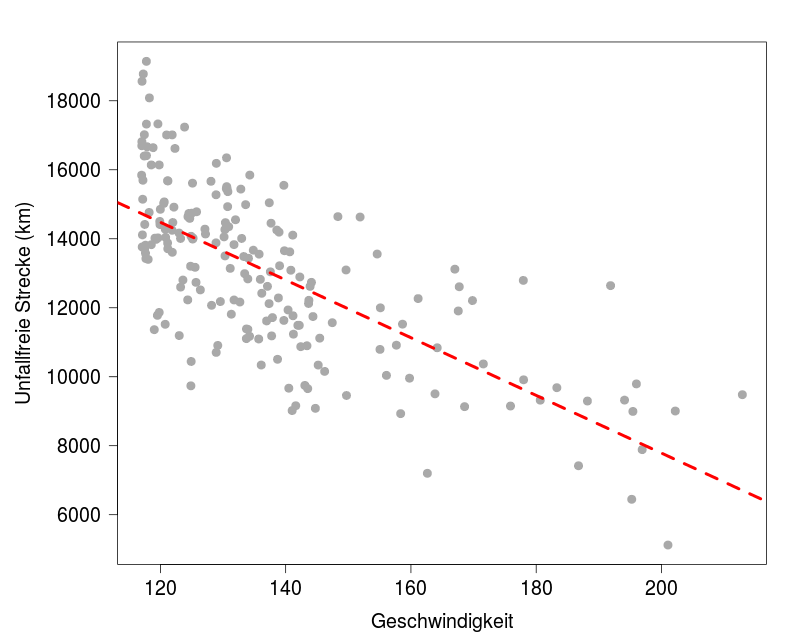
\includegraphics[width=1\textwidth]{chapters/svm/plot_lds.png}
\end{figure}

Es zeigt sich, dass schnelle Autofahrer tendenziell bereits nach einer kürzeren
Strecke einen Unfall haben. Die rote Gerade zeigt hierbei die vorhergesagten
Distanzwerte an, die allein durch Kenntnis der Variable Geschwindigkeit zu erwarten
sind. Die Gerade wird beschrieben durch die Gleichung:

\begin{equation*}
y = 24,516.56 - 83.65 \cdot Geschwindigkeit
\end{equation*}

Das lineare Modell sagt somit pro 1 km/h schnelleres Fahren etwa 84 weniger
unfallfrei gefahrene Kilometer vorher. Es ist jedoch deutlich zu erkennen, dass
allein das Wissen über die Geschwindigkeit keine allzu präzise Aussage über die
unfallfreie Strecke ermöglicht -- im Mittel liegt im vorliegenden Fall die absolute
Abweichung zwischen vorhergesagten und tatsächlichen Werten bei 1401 km. Ein
intelligentes System sollte bessere Prognosen erstellen, wenn seine Aufgabe die
Überwachung der Verkehrssicherheit ist! Um die Vorhersagegüte zu erhöhen, bieten sich
zwei Möglichkeiten an: Erstens können wir mehr aussagekräftige Prädiktoren in unser
Regressionsmodell aufnehmen. In diesem Fall würden wir das Modell zu einem
\textbf{multivariaten Regressionsmodell} erweitern. Zweitens könnten wir die
Komplexität der Modellgleichung erweitern, um auch nicht-lineare Schwankungen in den
Daten zu beschreiben.

\subsection{Nicht-lineare Regression}

Lineare Regressionsverfahren können erweitert werden, um auch nicht-lineare
Zusammenhänge zu beschreiben. Somit ergibt sich eine höhere Flexibilität,
Schwankungen in Daten abzubilden. Um nicht-lineare Zusammenhänge mithilfe der
\emph{linearen} Regression zu beschreiben, wird die Modellgleichung als Polynom
höherer Ordnung aufgestellt. Dabei bleibt die Gleichung linear in den Koeffizienten,
jedoch die Prädiktorvariablen gehen mit bis zu d-wertigen Polynomgrad in das
Regressionsmodell ein. Für ein Polynom d-wertiger Ordnung mit einer
Prädiktorvariablen \emph{x} sieht in die Regressionsgleichung somit wie folgt aus:

\begin{equation*}
y = \beta_0 + \beta_1 x + \beta_2 x^2 + ... + \beta_d x^d
\end{equation*}

Die allgemeine Koeffizientenlösung gilt auch für höherwertige Polynome, wobei in
diesem Fall für die Datenmatrix gilt X = $[1, x, x^2, ..., x^d]$, mit $\beta =
[\beta_0, \beta_1, \beta_2, ..., \beta_d]$:

\begin{equation*}
\beta = (X^TX)^{-1}X^Ty
\end{equation*}

Angenommen unser System möchte seine Vorhersagegenauigkeit verbessern und betrachtet
weitere Variablen, die mit dem Auftreten von Verkehrsunfällen auftreten können. Es
stellt fest, dass die Häufigkeit von Unfällen mit der Tageszeit zusammenhängt
(siehe Grafik 2.2).


\begin{figure}[!ht]
  \caption{Der Zusammenhang zwischen Uhrzeit und der Häufigkeit von Autounfällen pro
    Jahr.  Die rote Linie stellt den Schätzer der Unfallhäufigkeit durch eine
    einfache lineare Regression dar. }  \centering
  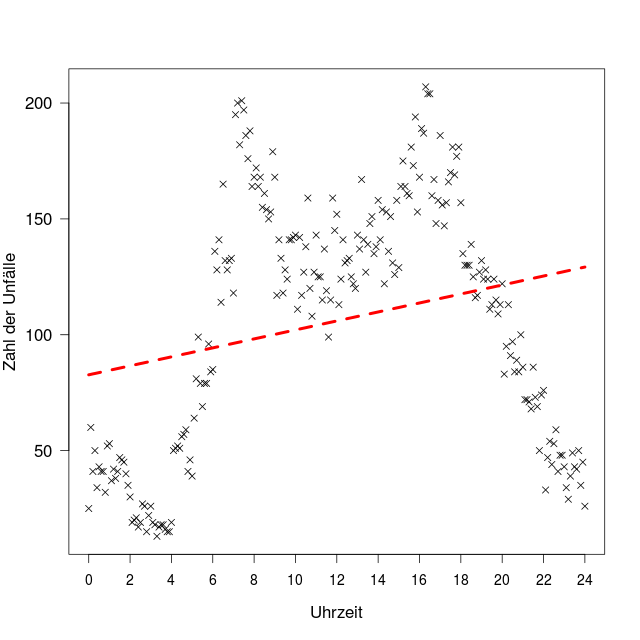
\includegraphics[width=1\textwidth]{chapters/svm/poly_1.png}
\end{figure}


Ein einfaches lineares Regressionsmodell ergibt einen geringen positiven Zusammenhang
zwischen Tageszeit und Zahl der Unfälle. Das Modell sagt somit die größte
Unfallwahrscheinlichkeit für 23:59 Uhr vorher und die geringste für 00:00 Uhr, was
eine sehr unplausible Vorhersage ist. Eine visuelle Inspektion der Daten ergibt
schnell, dass dieser einfache lineare Zusammenhang die Daten nicht adäquat
beschreibt. Eine Systematik in den Daten geht augenscheinlich darauf zurück, dass
sich nachts weniger Unfälle ereignen als tagsüber. Außerdem scheinen sich tagsüber
während der Zeit des Berufsverkehrs noch einmal etwas mehr Unfälle zu ereignen. Ein
Polynom zweiter Ordnung ist bereits in der Lage den U-förmigen Zusammenhang zwischen
Tageszeit und Unfällen darzustellen, der durch die Reduktion der Unfälle nachts
bedingt wird. Ein Polynom des 10. oder 20. Grades kann die Schwankungen abzubilden,
die auf den Berufsverkehr zurückgehen (siehe Grafik 2.3).

\begin{figure}[!ht]
  \caption{Der Zusammenhang zwischen Uhrzeit und der Häufigkeit von Autounfällen pro
    Jahr.  d ist der Grad der Polynomgleichung, die zur Vorhersage der
    Unfallhäufigkeit verwendet ist.}  \centering
  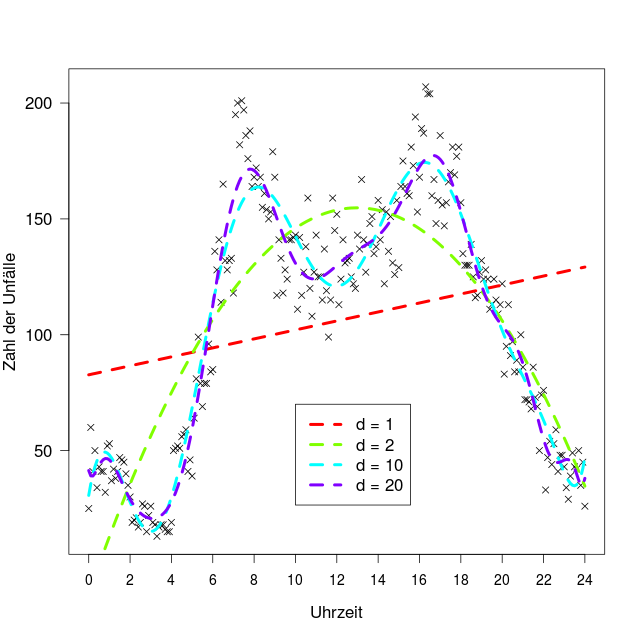
\includegraphics[width=1\textwidth]{chapters/svm/poly_2.png}
\end{figure}


Ist also anzunehmen, dass komplexere Modelle besser sind, da sie Daten genauer
beschreiben können und bessere Vorhersagen treffen? Sollte man in einer polynomialen
Regression immer anstreben den höchst-möglichen Polynomgrad zu modellieren, um die
Daten möglichst präzise abzubilden? Es gibt mehrere Gründe, die dagegen sprechen:
Erstens ist nicht zu erwarten, dass jegliche Erweiterung in der Komplexität auch
wirklich zu einer merklich verbesserten Vorhersageleistung führt. In dem Fall besagt
das philosophische Prinzip \emph{Ockhams Razor}, dass, wenn verschiedene Hypothesen
Daten gleich gut beschreiben, diejenige gewählt werden sollte mit, welche die
wenigsten Annahmen macht.  Ockhams Razor ist ein allgemeines Prinzip, welches nicht
nur in Regressionsproblemen Anwendung findet. In Grafik 2.3 ist zu erkennen, dass
ein Polynom 2. Grades die Daten schon wesentlich besser abbildet als der einfach
lineare Zusammenhang. Das Polynom 10. Grad ist wiederum ebenfalls eine Verbesserung,
da es Schwankungen, die auf den Berufsverkehr zurückgehen, abbildet. Es ist jedoch
fraglich, ob die Erhöhung der Komplexität von 10 auf 20 Polynomgrade wirklich
notwendig ist, um die Daten adäquat abzubilden. Nach Ockhams Razor wäre in dem Fall
das weniger komplexe Modell zu bevorzugen.

Des Weiteren besteht bei der Annahme eines zu komplexen Modells die Gefahr des
sogenannten \textbf{Overfittings}. Dieses bezeichnet den Umstand, wenn ein Modell
zwar vorgegebene Daten sehr gut beschreibt, aber nicht auf neue Testdaten
generalisiert, d.h. für solche Daten schlechte Vorhersagen macht, die nicht verwendet
wurden, um das Modell zu trainieren. Es ist wichtig, dass ein Modell auch für neue
Datenpunkte Aussagen treffen kann. Für unser Fahrsicherheitssystem wäre es fatal,
wenn es zwar alte Unfalldaten gut rekonstruieren kann, aber nicht zukünftige
Unfallgefahren voraussagen kann -- in dem Fall wäre es sogar vollends unnötig dieses
System überhaupt zu unterhalten.

Um bei der Erstellung eines Modells nicht auf Daten warten zu müssen, die erst in der
Zukunft (oder vielleicht niemals) gesammelt werden können, kann man eine sogenannte
\textbf{Kreuzvalidierung} durchführen: das vorhandene Datenset wird aufgeteilt in
einen \textbf{Trainings-} und einen \textbf{Testdatensatz}. Dies geschieht meistens,
indem ein bestimmter Prozentsatz der Daten zufällig dem Trainigsset und die anderem
dem Testset zugeteilt werden; eine Aufteilung von 80\% zu 20\% ist zum Beispiel
üblich. Anhand der Trainingsdaten werden die Regressionskoeffizieten geschätzt,
entscheidend für die Beurteilung eines Modells ist aber seine Fähigkeit die Testdaten
abzubilden. Dies ist ein allgemeines Prinzip, welches nicht nur bei linearer
Regression Anwendung findet. Im Falle einer Regression werden die Koeffizienten so
gewählt, dass sie den Trainingsdatensatz maximal präzise beschreiben. Durch
Annahme höherer Polynomgrade wird die Passung an den Trainingsdatensatz verbessert,
im Testdatensatz verschlechtert sich die Passung jedoch ab einem bestimmten
Komplexitätsgrad: ab hier geschieht Overfitting. Grafik 2.4 zeigt für den Uhrzeit--Unfallhäufigkeit Datensatz die Modellpassung verschiedener Polynomgrade anhand einer
Kreuzvalidierung. Es zeigt sich, dass Trainingsdaten mit steigendem Polynomgrad
besser vorhergesagt werden. Im Testdatensatz ist bei sehr hoher Komplexität jedoch
wieder eine Verschlechterung der Passung zu sehen. Beachtlich ist hierbei (sowohl für
Trainings- als auch Testdatensatz) die Verbesserung, die erzielt wird, wenn der
Polynomgrad von 1 auf 2 erhöht wird.

\begin{figure}[!ht]
  \caption{Das Ergebnis einer Kreuzvalidierung des Uhrzeit -- Unfallhäufigkeit
           Datensatzes. Gezeigt ist der Verlauf des mittleren Voraussagefehlers nach Komplexität
           des modellierten Polynoms für Trainings- und Testdatensatz.}  \centering
  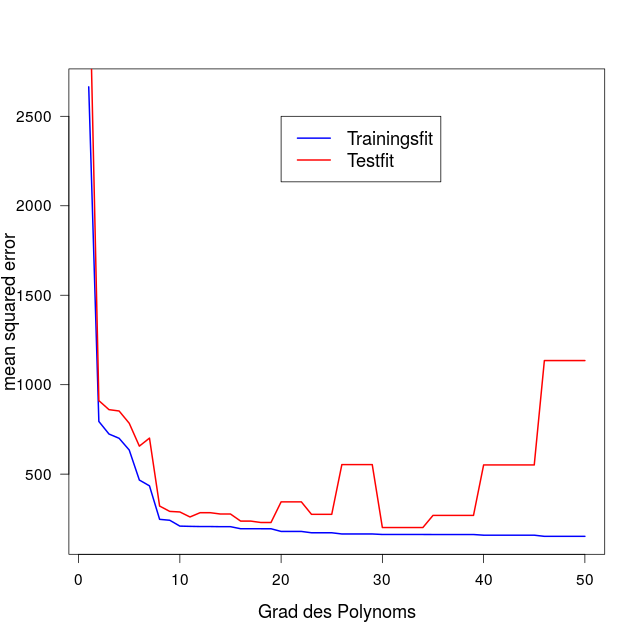
\includegraphics[width=1\textwidth]{chapters/svm/test_training.png}
\end{figure}

\subsection{Klassifikation}

Sehr häufig müssen in der Praxis qualitative Outcome-Variablen vorhergesagt
werden. Unser Fahrsicherheitssystem könnte beispielsweise der sehr relevanten Frage
nachgehen, unter welchen Umständen Verkehrsunfälle tödlich ausgehen. Beispielsweise
könnte es betrachten, ob durch Kenntnis des Gewichts und der Geschwindigkeit eines
Autos vorausgesagt werden kann, ob ein Unfall tödlich ausgeht. Grafik 2.5 zeigt für
100 verschiedene in Unfälle involvierte Autos das Gewicht und die Geschwindigkeit,
und ob der Unfall tödlich verlaufen ist. Es zeigt sich, dass eine höhere
Geschwindigkeit tendenziell mit tödlichem Ausgang einhergeht. Zu einem geringeren
Maße hängt auch das Gewicht mit der Tödlichkeit des Ausgangs zusammen. Ziel einer
Klassifikation ist eine Funktion zu finden, die auf Basis der Input-Werte das Label
schätzen kann. Hierbei wird eine Entscheidungsgrenze ("`decision boundary"')
angewendet; wenn der vorhergesagte Funktionswert über dieser Grenze liegt, wird eine
Klasse vorhergesagt, andernfalls wird die andere Klasse vorhergesagt. Wenn es möglich
ist die Klassen durch eine lineare Gleichung eindeutig voneinander zu trennen -- wie
in Grafik 2.5 der Fall -- nennt man das Problem \textbf{linear separabel}.
Verfahren, die zur Lösung von Klassifikationsproblemen verwendet werden, sind unter
anderem k nearest neighbor, lineare Diskriminanz Analyse, logistische Regression
Support Vector Machines oder neuronale Netze. Dabei können Support Vector Machines
und neuronale Netze sogar nicht-lineare Entscheidungsgrenzen abbilden.

\begin{figure}[!ht]
  \caption{Die Klassifikation eines Autounfalls als tödlich oder nicht tödlich in
    Abhängigkeit des Gewichts und der Geschwindigkeit des Autos. Die blaue Gerade ist
    eine sogenannte Entscheidungsgrenze ("`decision boundary"').} \centering
  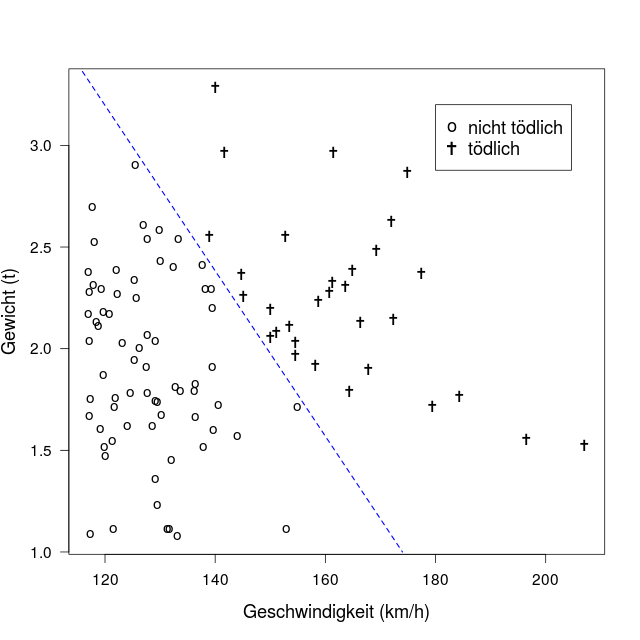
\includegraphics[width=1\textwidth]{chapters/svm/death_data.png}
\end{figure}

\section{Fazit \& Bewertung}

Methoden des statistischen Lernens können verwendet werden, um Computersystemen das
Lernen aus Beobachtungen zu ermöglichen. Die Fähigkeit zu lernen ist eine notwendige
Voraussetzung für maschinelle Systeme intelligentes Verhalten zu zeigen. Systeme
können aus großen Datenmengen Informationen integrieren, um zukünftige Ereignisse
oder Verhalten vorherzusagen. Maschinelles Lernen handelt sich um ein stark
wachsendes Forschungsfeld, das auch in der Öffentlichkeit mit viel Interesse verfolgt
wird -- nicht zuletzt aufgrund kürzlicher, medienwirksamer Errungenschaften
intelligenter Systeme, beispielsweise dem Erfolg des Systems AlphaGo, welches den
Weltmeister Lee Sedol im Go-Spiel überraschend bezwang. Lineare Regression wurde als
wichtiger Prototyp des statistischen Lernens ausführlicher vorgestellt. Dabei handelt
es sich um ein einfaches Verfahren, welches bereits gute Voraussagen liefert und auch
nicht-lineare Zusammenhänge darstellen kann. Auf fortgeschrittenere
Klassifikationsverfahren wie Support Vector Machines und neuronale Netze wurde ein
Ausblick gegeben. Einige grundsätzliche Prinzipien wie Ockams Razor und
Kreuzvalidierung gelten für jegliche Verfahren des statistischen Lernens, egal wie
komplex oder einfach sie erlernt werden können.

\section{Quellen und Literatur}
\begin{itemize}
\item James, G., Witten, D., Hastie, T., \& Tibshirani, R. (2013). \emph{An introduction to
statistical learning}. New York: Springer.

\item Legg, S., \& Hutter, M. (2007). A collection of definitions of intelligence. \emph{Frontiers
in Artificial Intelligence and applications}, 157, 17.

\item Lawrence N. (2016, May 09). Future of AI 6. Discussion of ``Superintelligence: Paths,
Dangers, Strategies'' [Web log post]. Retrieved from \newline
http://inverseprobability.com/2016/05/09/machine-learning-futures-6

\item Russell, S., \& Norvig, P. (2010) \emph{Artificial Intelligence: A modern approach
  (3rd. ed.)}. Upper Saddle River: Pearson.
\end{itemize}
